\section{System Overview}
Figure~\ref{fig:system_overview} displays the different components in the system and how they relate and communicate with each other.
% Tomas' system overview.
\begin{figure}[ht]
	\centering
	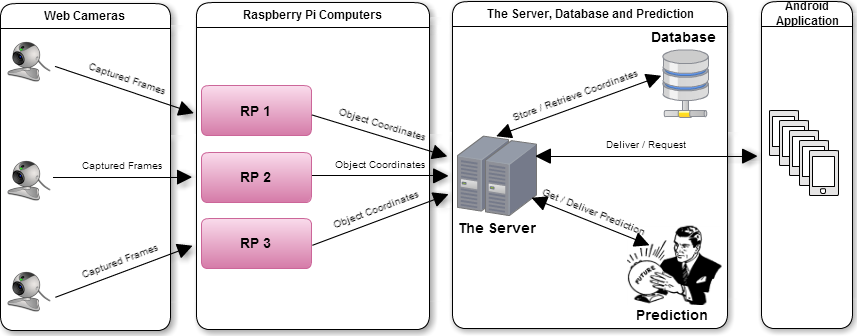
\includegraphics[scale=0.89]{system_overview/system_overview_tomas}
	\caption{Occupancy Analyzer System Overview}
	\label{fig:system_overview}
\end{figure}

As we can see, the system primarily consists of 4 components:

\begin{enumerate}
	\item Web cameras,
	\item Raspberry Pi computers,
	\item The server,
	\item and the Android application.
\end{enumerate}

All of these components are discussed further on in the respective chapters.

%camera placement and positioning reference: http://www.lorextechnology.com/support/self-serve/Camera-Location-Placement-and-Positioning/2700036
\section{Web Cameras}
The purpose of the web cameras is simply to surveillance the area they have been placed in and forward the captured frames to Raspberry Pi computers for further processing, as shown in Figure~\ref{fig:system_overview}. The cameras can be placed in a room, corridor, atrium or any other similar place in or outside of the building, where the services offered are required. Cameras can be placed either directly above the observed area (Figure~\ref{fig:camera_top}) or in the corner of it, as illustrated in Figure~\ref{fig:camera_corner}. Naturally, a camera placed above the observed area would give better results, since this increases its field of view and makes it easier to correctly detect and distinguish between multiple people walking side by side. Furthermore, for the best results one must also take many different factors into account, such as the distance between the camera and monitored area, environmental conditions of the area the camera is placed in, lighting conditions.

% Camera top placement.
\begin{figure}[ht]
	\centering
	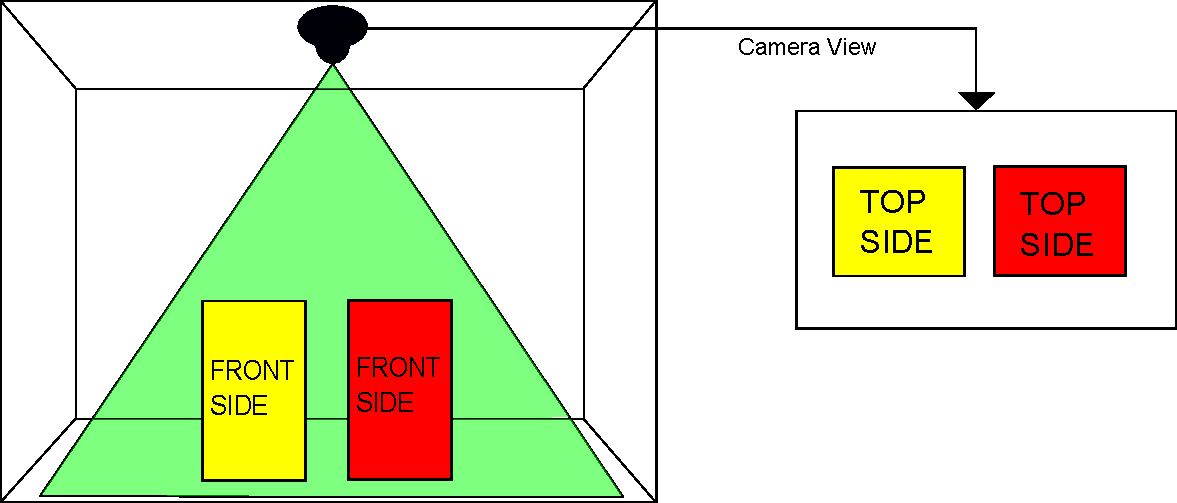
\includegraphics[scale=0.82]{camera_placement/camera_top}
	\caption{Camera top placement}
	\label{fig:camera_top}
\end{figure}

% Camera corner placement.
\begin{figure}[ht]
	\centering
	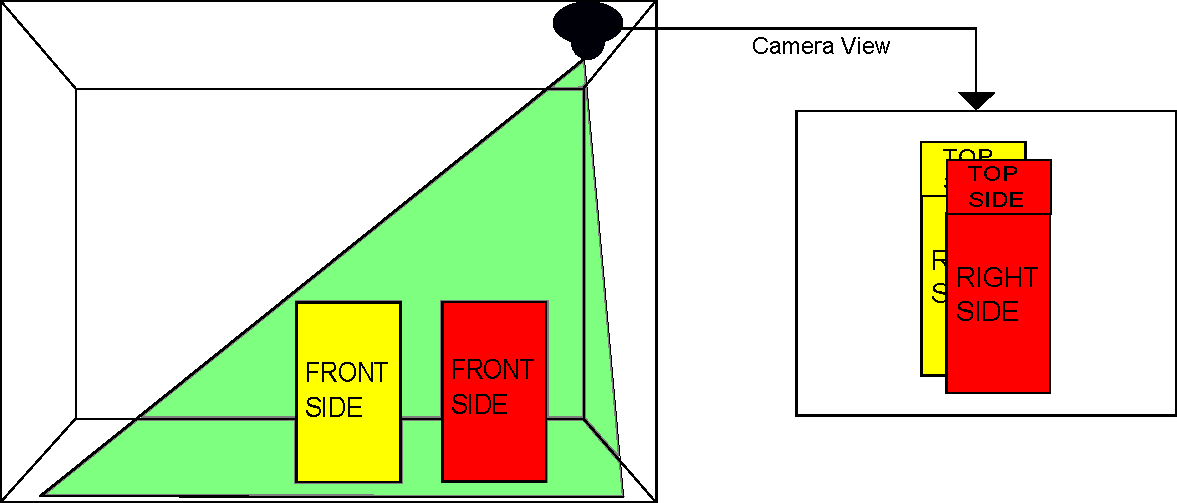
\includegraphics[scale=0.82]{camera_placement/camera_corner}
	\caption{Camera corner placement}
	\label{fig:camera_corner}
\end{figure}

\section{Raspberry Pi Computers}
The next component in the system architecture is Raspberry Pi computers. These computers have at least one web camera attached to them, and are responsible for processing the frames captured by these cameras. The main goal of processing these frames is to try to detect people in the monitored area and determine their position in that area. There are many different challenges in object detection, as well as various concepts and techniques that can be used to achieve this. We discuss these in the next sections.
	
	\subsection{Object Extraction}
	\label{sec:object_extraction}
	To detect and extract objects, or in our case, people and their movement, we need to apply several motion detection techniques on the frames we are receiving from the web camera. First of all, to detect changes in some monitored area, we naturally need to have at minimum two images, which we must compare to see what changes occurred. We will try to look into two different approaches in doing this, a simple one, and one that is a bit more complicated and sophisticated, but much more adaptive and flexible.
	
	\subsubsection{Simple Background Subtraction Approach}
	A simple approach - called Background Subtraction - would be to have a static background image of observed area that was taken prior to the analysis and did not have any people in it. Then, one can simply detect changes and movement in the area by subtracting the static background image from every newly taken image of the monitored area~\cite{background_subtraction_1}. The difference between the two images would then allow us to see if any changes happened, since after subtraction the resulting image would either be almost totally black (Figure~\ref{fig:background_subtraction_1}) - meaning no one walked passed the observed area - or the image would have some resulting bright contours of detected differences (Figure~\ref{fig:background_subtraction_2}).
	% Background Subtraction with no background changes.
	\begin{figure}[ht]
		\centering
		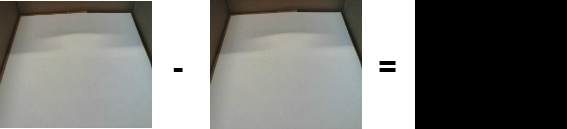
\includegraphics[scale=0.82]{background_subtraction/background_subtraction_1}
		\caption{Background Subtraction with no background changes}
		\label{fig:background_subtraction_1}
	\end{figure}
	% Background subtraction with background changes (lego man appearing).
	\begin{figure}[ht]
		\centering
		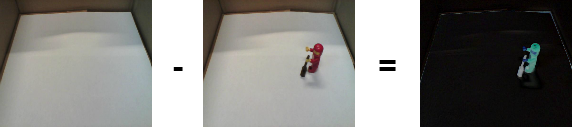
\includegraphics[scale=0.81]{background_subtraction/background_subtraction_2}
		\caption{Background Subtraction with background change}
		\label{fig:background_subtraction_2}
	\end{figure}
	
	After doing some research and experimenting with background subtraction technique, one will quickly discover that there are multiple weaknesses to it. 
	
	\begin{itemize}	
	\item First of all, if the initial background image is always static and never changes, this technique will fail in environments where lighting is dynamic. This is perfectly illustrated in Figure~\ref{fig:background_subtraction_3}. We can see that the lighting is much darker in the second image, possibly because the light was turned off in the monitored room, thus after subtracting our static background image from this image, the resulting image is simply a lighter version of the two images, and not the intended black image. The reason why this happens is because the original brighter background image has a much higher intensity, thus the average value of it's pixels are higher than the pixel values of the newly taken darker image. Naturally, this is a big problem, because now even if a person moves through the monitored area (Figure~\ref{fig:background_subtraction_4}), he or she will not be as easily extractable as in Figure~\ref{fig:background_subtraction_2}.
	% Background subtraction with background changes (lighting changes).
	\begin{figure}[ht]
		\centering
		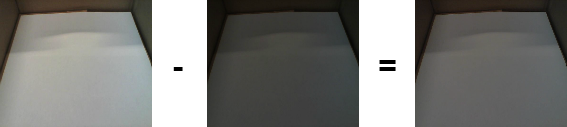
\includegraphics[scale=0.82]{background_subtraction/background_subtraction_3}
		\caption{Background Subtraction with background lighting change}
		\label{fig:background_subtraction_3}
	\end{figure}
	% Background subtraction with background changes (lighting changes + lego figure).
	\begin{figure}[ht]
		\centering
		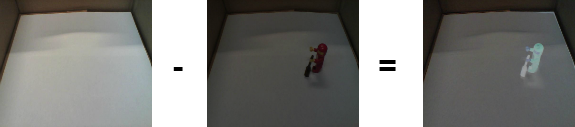
\includegraphics[scale=0.81]{background_subtraction/background_subtraction_4}
		\caption{Background Subtraction with background lighting change and lego figure appearing}
		\label{fig:background_subtraction_4}
	\end{figure}
	
	\item Another problem with background subtraction approach surfaces when a camera is placed inside an area which has objects that constantly change their original position (chairs, tables, appliances, etc.) by being moved, even small changes in object's location will spoil the resulting image after subtraction. As we can see in Figure~\ref{fig:background_subtraction_5}, the object is displayed twice in the resulting image, even though we were not even interested in it, making it much harder to detect actual people moving in the area. From now on, the resulting image after subtraction will always be corrupt unless the object is placed back in its original position.
		% Background subtraction with background changes (object changes location).
	\begin{figure}[ht]
		\centering
		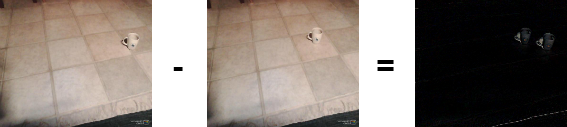
\includegraphics[scale=0.82]{background_subtraction/background_subtraction_5}
		\caption{Background Subtraction with object changing it's location}
		\label{fig:background_subtraction_5}
	\end{figure}
	\end{itemize}
	
	In conclusion, we can see that simple background subtraction approach can work well in static environments, however it falls short in dynamic spaces. Naturally, these mentioned drawbacks of background subtraction approach need to be handled for object detection to work well, which creates additional challenges when implementing the system.

	\subsubsection{Running Average Approach}
	\label{sec:running_average_approach}
	A much better approach for movement detection is using a running average method. In this technique we do not need to rely on a static background image of the monitored area taken prior to analysis. Instead, we try to find a new "approximate" background image by interpreting any changes in the background as noise and blurring them out. This is accomplished by taking a train sequence of multiple previously captured frames and performing arithmetic averaging on that sequence~\cite{running_average_approach_1}. This exact approach is illustrated in Figure~\ref{fig:running_average_example}. As we can see, hand motion moving up and down (Figures~\ref{fig:running_average_1},~\ref{fig:running_average_2} and~\ref{fig:running_average_3}) gets blurred out when applying running average method, thus producing an approximate background image (Figure~\ref{fig:running_average_4}) that can be used for subtraction of the test frames from it. This method of object extraction works very well and has a lot of flexibility. It can adapt to environmental changes in the monitored area, thus eliminating most of the weaknesses that the background subtraction approach has. For these reasons, the running average approach was chosen for our design.
	% Running average example.
	% subfigure allows to group figures and put them next to each other.
	\begin{figure}[ht]
		\centering
		\subfigure[Test frame 1]{
		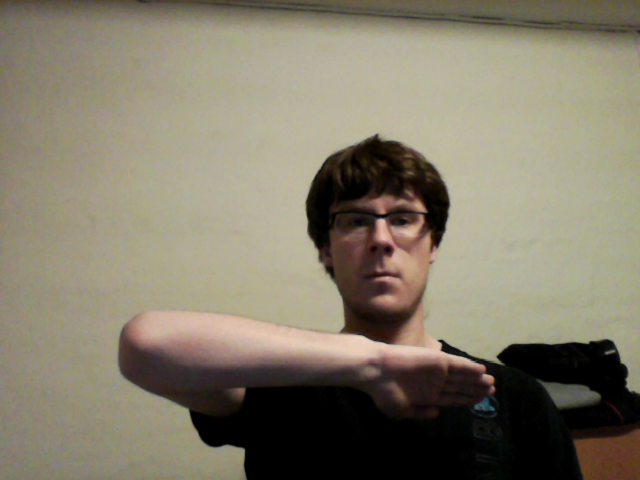
\includegraphics[scale=0.40]{running_average/running_average_1}
		\label{fig:running_average_1}}
		\quad
		\subfigure[Test frame 2]{
		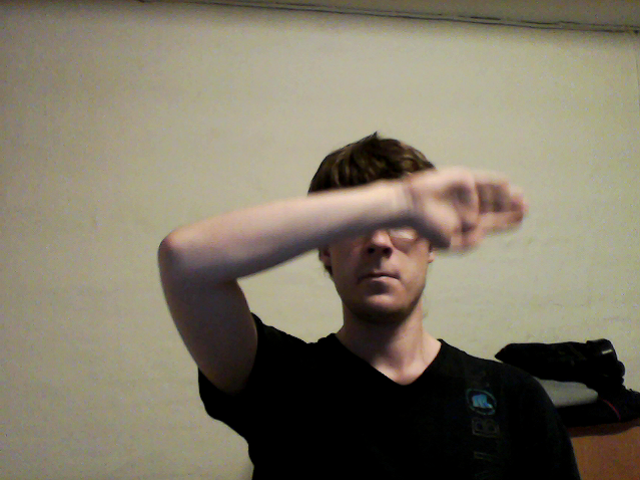
\includegraphics[scale=0.40]{running_average/running_average_2}
		\label{fig:running_average_2}}
		\subfigure[Test frame 3]{
		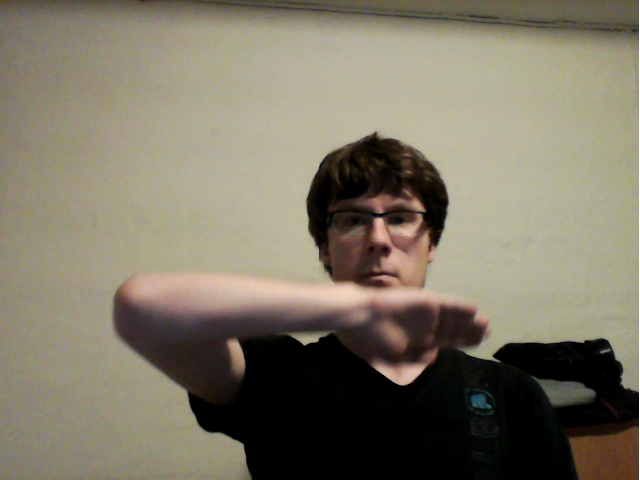
\includegraphics[scale=0.40]{running_average/running_average_3}
		\label{fig:running_average_3}}
		\quad
		\subfigure[Running Average frame]{
		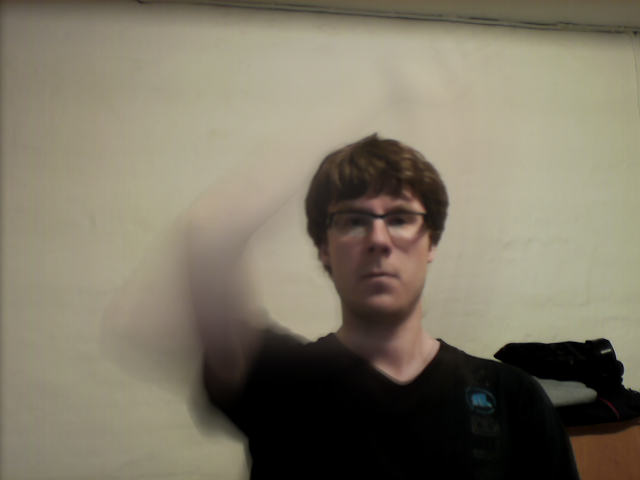
\includegraphics[scale=0.40]{running_average/running_average_4}
		\label{fig:running_average_4}}
		\caption{Example of Running Average technique}
		\label{fig:running_average_example}
	\end{figure}
	\subsection{Object Detection}
	\label{object_detection}
	Now that we can extract objects using running average technique, we need to be able to actually find them in the resulting image we get after we perform subtraction. For this, we need to apply several key techniques in image processing. 
	
	\begin{itemize}
	\item After we capture the initial frame of the monitored area, it will often contain noise and small details that we are not interested in. To deal with this, we must first apply blur or smoothing filter. In blurring technique we calculate weighted averages of areas of pixels in a source image by passing through it~\cite{blur_1}, which helps to reduce image noise and detail, as shown in Figure~\ref{fig:blur_example}.
	% Blur example.
	\begin{figure}[ht]
		\centering
		\subfigure[Original frame]{
		
\includegraphics[scale=0.40]{blur/blur_1}
		\label{fig:blur_1}}
		\quad
		\subfigure[Frame after blur is applied]{
		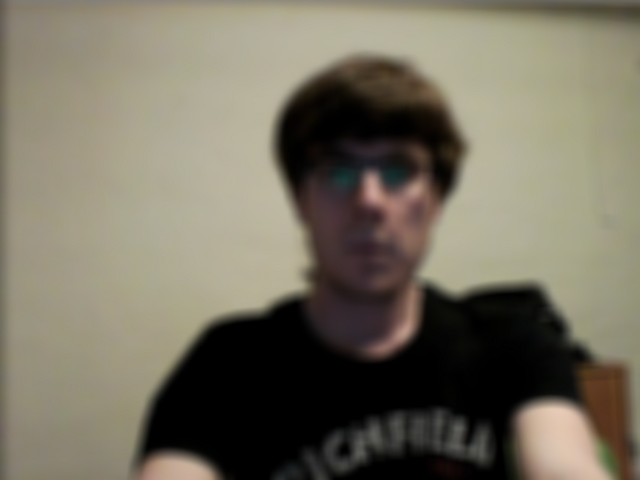
\includegraphics[scale=0.40]{blur/blur_2}
		\label{fig:blur_2}}
		\caption{Blur example}
		\label{fig:blur_example}
	\end{figure}
	
	\item After we remove the initial noise, we can perform subtraction using running average approach (described in Section~\ref{sec:running_average_approach}). After subtraction we will either get a nearly totally black image, meaning no motion occurred, or an image where some colors stand out, meaning some motion has occurred. 
	
	\item In either case, for further processing of the taken frame, we can choose to convert it to a grayscale image. The reason for this is that the original RGB image we get has three channels, while grayscale image has only one~\cite{grayscale_1}, thus it is easier to work with. This procedure is illustrated in Figures~\ref{fig:grayscale_1},~\ref{fig:grayscale_2} and~\ref{fig:grayscale_3}. 
	
	\item For further processing of the image, we apply threshold technique, which converts the image to black and white and removes some more unwanted details and noise~\cite{threshold_1}. After threshold is applied we get the image shown in Figure~\ref{fig:threshold_1}. 
	
	\item Moreover we want to expand the interesting parts of the image and contract smaller pieces, which can be considered noise and managed to slip through, even after we performed thresholding. To do so, we use two fundamental operations in morphological image processing, that is, dilation and erosion. Dilation allows us to expand the shapes contained in the image~\cite{dilation_1}, whereas erosion simply shrinks shapes~\cite{erosion_1}, so that bright regions surrounded by dark regions shrink in size, and dark regions surrounded by bright regions grow in size. When we apply dilation and erosion we get the image shown in Figure~\ref{fig:dilate_erode_1}. 
	
	\item Now, to project the detected area onto the original frame, we simply use bounding box technique, which gives us the coordinates of the rectangular border that fully covers the extracted white silhouette~\cite{bounding_box_1} that we got in~\ref{fig:dilate_erode_1}. Then we use these coordinates to draw a simple rectangle around the extracted object, as well as mark it's middle position by a red circle, as illustrated in Figure~\ref{fig:bounding_box_1}.
	\end{itemize}
	\begin{figure}[ht]
		\centering
		\subfigure[Original frame]{
		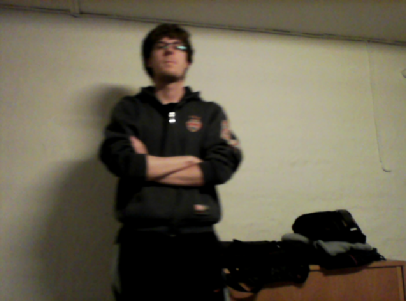
\includegraphics[scale=0.65]{grayscale/grayscale_1}
		\label{fig:grayscale_1}}
		\quad
		\subfigure[After subtraction]{
		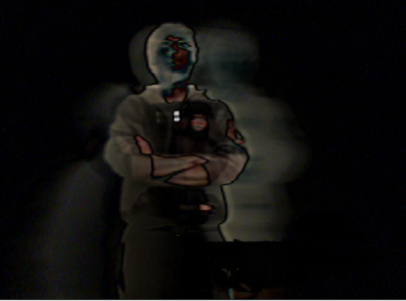
\includegraphics[scale=0.65]{grayscale/grayscale_2}
		\label{fig:grayscale_2}}
		\subfigure[After grayscale filter is applied]{
		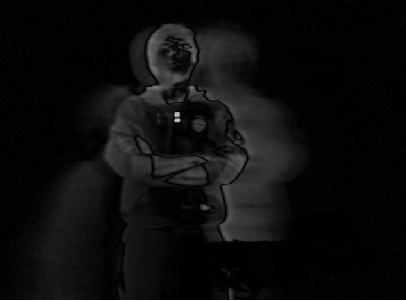
\includegraphics[scale=0.65]{grayscale/grayscale_3}
		\label{fig:grayscale_3}}
		\quad
		\subfigure[After threshold is applied]{
		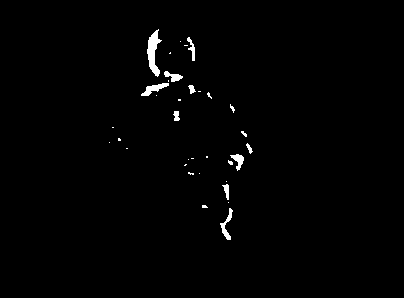
\includegraphics[scale=0.65]{threshold/threshold_1}
		\label{fig:threshold_1}}
		\subfigure[After dilation and erosion]{
		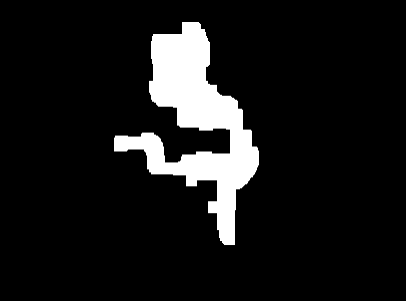
\includegraphics[scale=0.65]{dilate_erode/dilate_erode_1}
		\label{fig:dilate_erode_1}}
		\quad
		\subfigure[After bounding box is drawn]{
		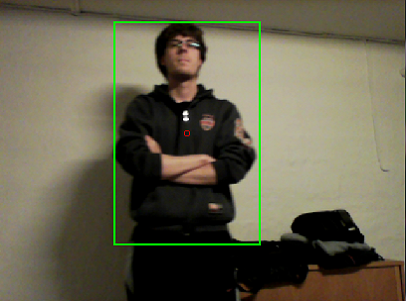
\includegraphics[scale=0.65]{bounding_box/bounding_box_1}
		\label{fig:bounding_box_1}}
		\caption{Object detection example}
		\label{fig:object_detection_example}
	\end{figure}
	
	In conclusion, by applying the steps discussed in this section, we can fairly accurately detect people and their movement in the monitored area.
	
	\subsection{Object Differentiation}
	\label{object_differentiation}
	There will naturally be cases when multiple people will walk through the monitored area and will be captured by the cameras, therefore we must have a way to differentiate between them. This task becomes rather difficult if people are very close to each other, since they will simply be interpreted as one person. However, as long as people are far enough from each other, the task becomes significantly easier. There are multiple ways of differentiating between objects. 
	
	One of them is to simply look at the objects histogram, which gives a graphical representation of the intensity distribution of pixels~\cite{histogram_1}. Since people are usually dressed in different color clothes, we can simply calculate a histogram for every detected person and remember it. Now, every time we receive a new frame and detect a person in it, we go through our previously saved histograms and check whether any of them are the same as our newly detect persons histogram. If there is such histogram, we interpret the person we detected in our new frame as the same person we detected in the last, otherwise, we conclude that we have not detected this person before, thus save his histogram for future reference. The biggest weakness of this approach is that a person's clothes might have different colors from the front and back. Therefore, his histogram calculated while he is facing the camera might be rather different than the histogram of when his back was towards the camera. For this reason, if the person decides to turn around midway, he might be interpreted as a new person - never seen before by the camera - when in fact his frontal or back histogram was already saved. 
	
	Another approach of differentiating between multiple people, and in fact the approach we used in our design, is to simply use the whole frame as a coordinate system and remember the last coordinate of every single detected person. Now, similarly to histogram approach, whenever we detect a new person in the frame, we simply look throughout previously saved coordinates, and if we find that this new person's coordinates is relatively close to some previously saved person's coordinates, we simply interpret him as the same person we detected a second or or few seconds ago, otherwise we see him as a new person. Naturally, we must regularly clear our previously saved coordinates, so that newly arrived person would not simply, by taking a similar path, be interpreted as a person who is no longer in the monitored area. This approach of differentiating between people is is illustrated in Figure~\ref{fig:object_differentiation_example}.
	
\begin{figure}[ht]
		\centering
		\subfigure[One person enters the monitored area]{
		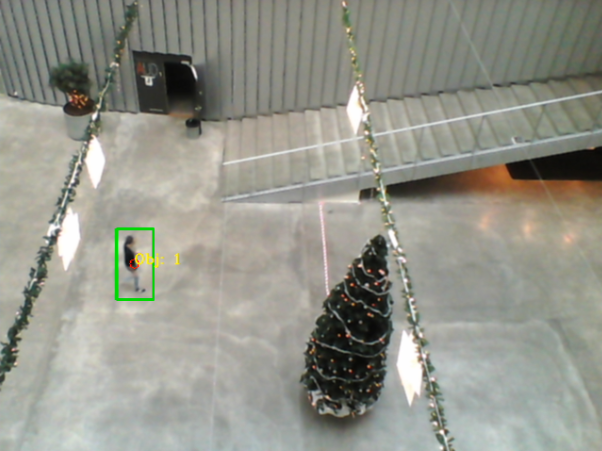
\includegraphics[scale=0.48]{object_differentiation/1}
		\label{fig:object_differentiation_1}}
		\quad
		\subfigure[Second person enters the monitored area]{
		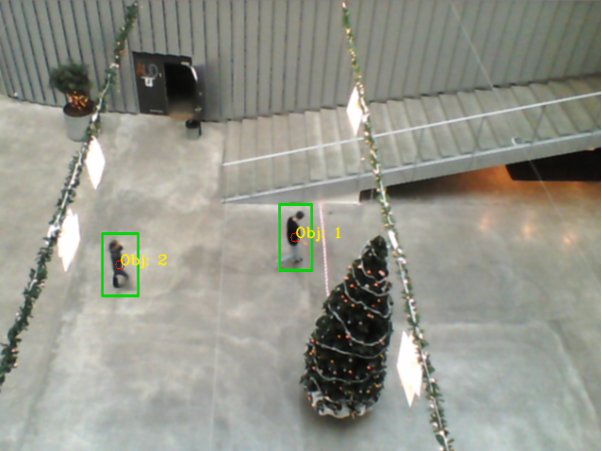
\includegraphics[scale=0.48]{object_differentiation/2}
		\label{fig:object_differentiation_2}}
		\subfigure[Two people continue their walk through the monitored area]{
		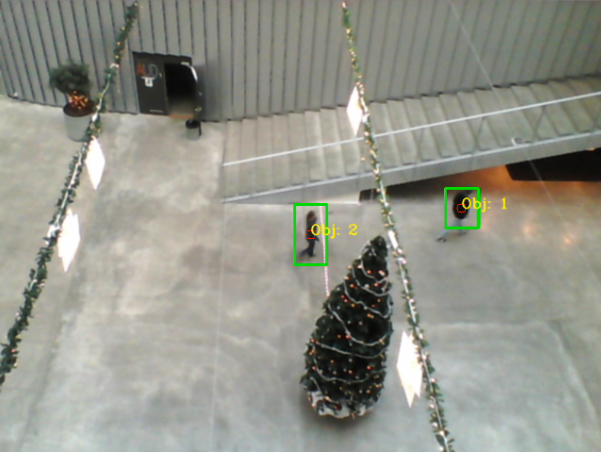
\includegraphics[scale=0.48]{object_differentiation/3}
		\label{fig:object_differentiation_3}}
		\quad
		\subfigure[First person leaves the monitored area]{
		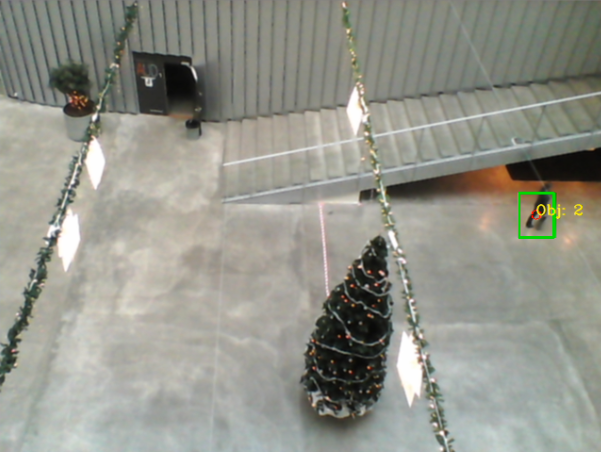
\includegraphics[scale=0.48]{object_differentiation/4}
		\label{fig:object_differentiation_4}}
		\caption{Object differentiation example in the monitored area}
		\label{fig:object_differentiation_example}
	\end{figure}




\section{The Server}
{\color[rgb]{1,0,0} \textbf{\large TODO}}

The server is the central part of the whole system. It is here the Raspberry PIs send all the gathered data, where data are stored and structured, and where Android devices can fetch information about rooms, people, and predictions on which exits a person is most likely to use.

The server is thus split into the following parts:

\begin{enumerate}
	\item Data Input API,
	\item Data Output API,
	\item Storage.
\end{enumerate}

% discuss why it is structured in this way and not p2p

\subsection{Data Input API}
All sorts of devices can be used to capture and process data. To simplify the process and to allow access for all types of devices, the server provides an API which allows the senders to focus on data capturing and processing.

\subsection{Data Output API}
As with the devices providing the data for the server, the devices which requests data from the server can be of different types. By providing an API these devices can focus on how to use and present the data, and let the server focus on how the data is fetched. This ensures that all data is available for everyone and that each request has a minimum of effect on other devices access to the data.

\subsection{Storage}

\section{Prediction}

\subsection{Gathering statistical data}
\label{ssub:statisticaldata}
In addition to storing data about each occupant we also store data about how occupied each section of the recorded image is. The process is simple; we split the image of a room into sections, referred to as cells, and each time an occupant enters a cell the stored activity for the given cell is increased. Each room has a different and independent set of cells. This data tells us which sections of the room are most occupied. We use the activity data to perform predictions about an occupant's future actions using a custom prediction model.

\subsection{Custom prediction model based on HMM}
\label{ssub:designcustomprediction}
We have chosen to build our own prediction model heavily inspired by the hidden Markov model. Each cell in the image is a state where the state transition probability is the likelihood of an occupant moving to an adjacent cell and the output probability is the likelihood of an occupant going to an exit given any current cell. Unlike a regular hidden Markov model, we do not store probability values individually for each state, but rather do the necessary calculations each time a prediction is requested by using the stored activity values of each cell. Additionally, our custom model allows us to take several custom factors into account during calculations. These factors work as a rule set for likely or unlikely occupant actions:
\begin{itemize}
\item An occupant entering a room from a given exit is less likely to exit the room at the given exit.
\item An occupant is more likely to continue moving in his general direction and least likely to return to his previously visited cell.
\item An occupant is more likely to move to the adjacent cell with the highest amount of previous activity.
\item The likelihood of an occupant exiting at a given exit (unless it also serves as the occupant's entrance) is inversely proportional to the direct distance to the given exit, producing a magnet-like effect. 
\end{itemize}
These factors have an influence on a final value of a cell or exit, which is used when calculating each probability. The sum of the probabilities of an occupant moving to each individual exit given a current cell is 100. The cell with the highest probability will be the predicted cell.
\begin{figure}[ht]
\centering
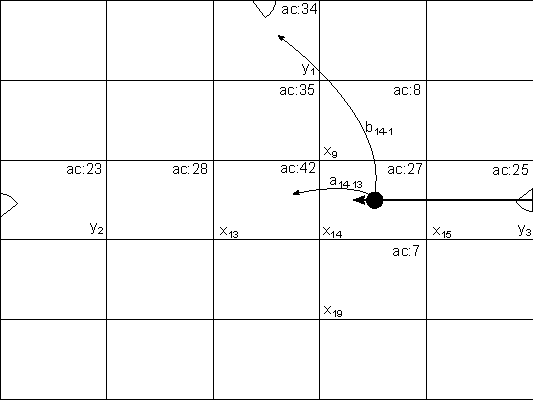
\includegraphics{prediction_figures/custom}
\caption{Applying the custom model to a scenario.}
\label{fig:custom_model}
\end{figure}

Figure \ref{fig:custom_model} shows the custom model translated to a scenario. Each cell contains an identification number, an activity count and a value denoting whether or not the cell is an exit cell. The occupant entered the room at exit \(y_3\) and the current state is \(x_{14}\). \(a_{14-13}\) denotes the state transition probability of the occupant moving from state \(x_{14}\) to state \(x_{13}\). \(b_{14-1}\) denotes the output probability of the occupant ultimately choosing exit \(y_{1}\). Taking our custom rule set into account, the occupant is least likely to exit at \(y_3\) and most likely to continue to \(x_{13}\). Moving to \(x_9\) would increase the probability of the occupant exiting at \(y_{1}\) (\(b_{9-1}\)) significantly.

\section{Android Application}
{\color[rgb]{1,0,0} \textbf{\large TODO}}